\chapter{Cold atomic gases}
\label{cha:cold-gases}

\section{Bose-Einstein condensation}
\label{sec:BEC}


\paragraph{BEC in noninteracting gas}
In 1925, Albert Einstein (prompted by the earlier work of the indian
polyglot Satyendra Nath Bose) considered what would happen to a
non-interacting bosonic gas of non-relativistic particles in the
thermodynamic limit, as one lowers the temperature. He predicted the
phenomenon we now call \textit{Bose-Einstein condensation} (BEC),
namely a phase transition, below a critical temperature $T_c$, to a
new state of matter, in which a finite fraction of all the particles
would occupy the same single-particle state. In particular, if we take
$N$ particles in a cubic box of volume $L^3$, then they would
predominantly occupy the zero-wavevector state $\kv = 0$, and the
critical temperature would be~\cite{9780198507192}
%
\begin{equation}\label{eq:Tc3D}
  T_c \simeq 3.31 \frac{\rho^{2/3}\hbar^2}{m k_B}
\end{equation}
%
with the density $\rho = N/L^3$ and $m$, $k_B$ being the particle
mass and Boltzmann's constant, respectively.

At its core, BEC is a statistical phenomenon, steming from the
indistinguishability of elementary particles in quantum field theory,
coupled to the ``spin-statistics'' theorem, which sets a constraint on
the symmetry of the many-body wavefunction regarding the interchange
of its arguments. In fact, one can hand-wavingly deduce the
temperature below which quantum degeneracy would start playing a role
in a many-body system, by arguing that the thermal de Broglie
wavelength should be comparable to or greater than the inter-particle
distance (which in our case is $\rho^{-1/3}$ on
average)~\cite{Leggett_1999}. Apart from the numerical prefactor, we
get the same answer as Eq.~\eqref{eq:Tc3D}. While one may argue that
elementary massive bosons do not exist, it is worth emphasizing that
indistinguishability only plays a role when there is a finite
probability for exchange processes to occur between the particles. In
that sense, all odd-isotope alkali atoms under relevant experimental
conditions (see below) effectively behave as bosons: their many-body
wavefunction is symmetric under the exchange of any two such atoms.

\paragraph{BEC in interacting system}
Interestingly enough, BEC was considered by many at the time to be a
pathological behaviour of the non-interacting gas, which would resolve
once interactions were properly accounted for. In fact, it is well
known that the ideal Bose gas has infinite compresibility. Since most
experimental systems found in nature are interacting ones, one needs
to explore the notion of BEC in an interacting system. In order to
proceed however, we must first introduce the key concept of
\textit{single-particle density matrix}.

\paragraph{One-body density matrix}
Following Leggett, we characterise each of the $N$
particles\footnote{The particles are assumed to be spinless, for
  simplicity; the extension to particles posessing a nontrivial
  internal degree of freedom is straightforward.} by a position vector
$\rv_i$, with the label $i$ running from 1 to $N$. Any pure state $s$
of the (now interacting) system -- which can be also subjected to an
external potential -- can be described at time $t$ by the many-body
wavefunction $\Psi_s(\rv_1,\rv_2,\dots,\rv_N,t)$. Therefore, the most
general state of the system (also called \textit{mixed state}) can be
written as a superposition of pure orthonormal states $s$ with
different weights $p_s$. The single-particle density matrix
$\hat{\rho}_1(\rv,\rv^{\prime},t)$ then represents the probability
amplitude, at time $t$, of finding a specific particle at position
$\rv$, multiplied by the amplitude of finding it at $\rv^{\prime}$,
and averaged over the positions of all the other particles:
%
\begin{align}\label{eq:one-particle-rho}
  \hat{\rho}_1(\rv,\rv^{\prime},t) & \equiv N \sum_s p_s \int d\rv_2d\rv_3\dots
d\rv_N
\Psi_s^{\star}(\rv,\rv_2,\dots,\rv_N,t)\Psi_s(\rv^{\prime},\rv_2,\dots,\rv_N,t)\nonumber\\
& = \sum_i n_i(t) \phi_i^{\star}(\rv,t) \phi_i(\rv^{\prime},t)
\end{align}
% 
where in the second line we have re-written the density matrix in
diagonal form, introducing its eigenvalues $n_i$ and eigenvectors
$\phi_i$, which form a complete orthonormal set at any time $t$ (here
$i$ labels a good quantum number of the problem, i.e. momentum in a
translationally-symmetric situation).

\paragraph{Penrose-Onsager criterion for BEC}
We are now ready to state the Penrose-Onsager criterion for
condensation, first formulated in 1956: if at any given time $t$ it is
possible to find a complete orthonormal basis of states of
$\hat{\rho}_1$ such that one and only one of these states has an
eigenvalue of order $N$ (the rest being of order 1), then we say the
system exhibits BEC. One should note that this definition only applies
to ``simple'' BEC, as opposed to the ``fragmented'' case (of no
concern to us here), where two or more of the eigenvalues of the
one-body density matrix are of order $N$.

\paragraph{Condensate wavefunction and the order parameter}
We denote the single macroscopic eigenvalue of the density matrix by
$N_0(t)$, and its corresponding eigenfunction by
$\phi_0(\rv,t)$. $\phi_0$ is called the \textit{condensate
  wavefunction} and the $N_0$ particles occupying it the
\textit{condensate}, while the ratio $N_0/N$ is the \textit{condensate
  fraction}. It is not necessarily true that $N_0 = N$, even at zero
temperature. Also note that, while $\phi_0$ behaves as a
single-particle Schr\"{o}dinger wavefunction, it is generally not an
eigenfunction of the single-particle part of the Hamiltonian, or of
any other simple operator for that matter, other than
$\hat{\rho}_1$. Another useful quantity frequently found in the
literature is the so-called \textit{order parameter},
$\psi(\rv,t) = \sqrt{N_0(t)}\phi_0(\rv,t)$. We see that, while
$\phi_0$ is normalized to 1, $\psi$ will be normalized to $N_0(t)$.

\paragraph{No-go theorem for lower dimensionality}
Before moving on to relevant experimental results, it is worth
mentioning the existence of a ``no-go'' theorem, due to Hohenberg,
stating that, in the thermodynamic limit, BEC cannot occur at a finite
temperature in any system moving freely in space in less than three
dimensions, irespective of the existence and/or sign of the
interparticle interactions. Note that this theorem, however, only
applies under equilibrium conditions, the nonequilibrium case still
being an open question.  Furthermore, there is no general proof that a
realistic system of interacting bosonic particles must show BEC, even
at zero temperature -- the solid phase of ${}^4$He constitutes an
obvious counter-example.

\paragraph{Experimental proof}
Most gases, with the notable exception of ${}^4$He, are solids at the
densities and temperatures predicted by Eq.~\eqref{eq:Tc3D}. That is
why it took no less than 70 years between Einstein's original paper
and the first experimental observation of BEC in an atomic gas. In
1995, the group of Eric Cornell and Carl Wieman succesfully condensed
a cloud of ${}^{87}$Rb atoms, by first bringing the system to a very
low density, and then cooling it fast enough to prevent any
recombination processes that would have lead to the formation of the
solid phase. While other odd-isotope alkali elements, especially
${}^{23}$Na or ${}^{7}$Li, are also routinely used in experiments, the
first non-alkali atom to be cooled into the BEC phase was hydrogen
${}^1$H. Due to the extreme diluteness of these systems
($\rho < 10^{15}$ atoms/cm${}^3$), the typical range of $T_c$ is from
$20$ nK to a few $\mu$K. Achieving such ultra-low temperatures
stimulated the development of novel experimental techniques, such as
magnetic/laser trapping and evaporative cooling of atoms.

\paragraph{Diagnostic techniques}
The very low densities of alkali gases also limit the range of
available diagnostic techniques. The most commonly employed method in
BEC experiments is optical absorption imaging, where one shines a
laser on the gas and detects the percentage of transmitted power. The
image is usually taken after removing the trap and allowing the gas to
expand. This gives information about the gas density as a function of
coordinates and time, with a spatial resolution of a few $\mu$m. In
stark contrast to liquid ${}^4$He, density-related information seems
to be sufficient for most practical purposes.

\paragraph{Diluteness/weak interaction condition}


\section{Gross-Pitaevskii equation}
\label{sec:GPE}

\paragraph{Short history and utility of GP equation}
As it turns out, many of the experimental results in ultracold gases
can be interpreted on the basis of a single equation for the
condensate wavefunction $\phi_0(\rv,t)$. This equation, first derived
in 1961 independently by Eugene Gross and Lev Pitaevskii, was
originally intended as a phenomenological description of quantum
vortices in the superfluid phase of liquid ${}^4$He, below the lambda
point. Since liquid helium is a strongly interacting system however,
the GP equation turned out to be much better suited to alkali gases.
Before giving the concrete formulation of the GP equation, we must
first explore the nature of the inter-atomic interactions.

\paragraph{s-wave scattering length}
In dilute systems, the inter-atomic distance $d = \rho^{-1/3}$ is on
the order of 1000~\AA, while the range $r_0$ of the inter-atomic
potential, namely the extent of the last bound state of the van der
Waals interaction, is about 50-100~\AA. As $d \gg r_0$, the
probability of three-atom colissions is substantially diminished. This
justifies limiting ourselves to a binary (instead of three-body or
more) scattering problem: consider two atoms, separated by a relative
distance $r$ and interacting in three dimensions through a potential
$V(r)$. We can therefore decouple their center-of-mass motion from
their relative one and write a Schr\"{o}dinger equation for the
scattering states $\psi(r)$.

For temperatures below $T_c$, the thermal de Broglie wavelength
$\lambda_T > d$ (as mentioned in Sec.~\ref{sec:BEC}), meaning all
significantly occupied states will have small wavevectors,
$k \ll r_0^{-1}$. This directly translates to a low relative kinetic
energy, and hence small relative wavevectors, for the scattering
problem outlined above. However, we know from scattering theory that
the probability for two atoms, with relative angular momentum $\ell$,
of being separated by a distance $r \ll k^{-1}$ is proportional to
$(kr)^{2\ell}$, therefore essentially negligible in the limit
$k r_0 \ll 1$. That is of course, unless $\ell = 0$, meaning their
relative state is $s$-wave, which is what we will assume from now
on. Since $r_0 \ll d$, one can use the asymptotic expression for
$\psi(r)$, which only depends on the scattering amplitude. At small
wavevectors, this amplitude can be safely replaced by the
\textit{$s$-wave scattering length} $a_s$, which will encapsulate all
the interaction effects on macroscopic properties of the atomic gas.

One can now replace the two-body potential $V(r)$ with an effective
interaction, $V_{\text{eff}}(r)$, provided it gives the same
scattering length. The limit of small wavevectors prompts us to only
consider the lowest Fourier component of $V_{\text{eff}}$, equivalent
in real space to a contact interaction\footnote{Technically, one
  should also include a regularizing part in order to remove any $1/r$
  divergencies of the wavefunction.}
$V_{\text{eff}}(r) = g \delta(r)$, where we have introduced the
interaction coupling constant $g$, whose value can be calculated using
the first-order Born approximation~\cite{9780198507192} 
%
\begin{equation}\label{eq:g-constant}
  g = \frac{4\pi\hbar^2}{m} a_s
\end{equation}
% 
The scattering length $a_s$ therefore becomes the small parameter of
the theory of weakly-interacting ultracold gases, and the validity of
the Born approximation rests on the following two conditions
%
\begin{align}
  k \abs{a_s} & \ll 1\\
    \abs{a_s} & \ll \rho^{-1/3}\label{eq:diluteness-condition}
\end{align}
% 
Eq.~\eqref{eq:diluteness-condition} is called the ``diluteness
condition'', and it paves the way to various mean-field approaches,
such as the GP equation.


\paragraph{Derivation of Gross Pitaevskii equation}
Formally, the GP equation corresponds to the lowest-order expansion in
$a_s$ of the more exact Bogoliubov theory. However, we will try to
give a hand-waving justification of it for the zero-temperature
case. At $T=0$, all $N$ particles are in the condensate, therefore one
could neglect all inter-particle correlations and introduce the
simplest (Hartree-Fock) ansatz, expressing the ground state many-body
wavefunction $\Psi$ in the symmetrized form
%
\begin{equation}\label{eq:HF-ansatz}
  \Psi(\rv_1,\rv_2,\dots,\rv_N,t) = \prod_{i = 1}^{N} \phi_0(\rv_i,t)
\end{equation}
% 
As explained in Sec.~\ref{sec:BEC}, the single-particle state $\phi_0$
(now occupied by all the bosons) obeys a Schr\"{o}dinger-like
equation, to which we must add the energy of the effective binary
interactions. In mean-field, these interactions contribute the
equivalent of a one-particle potential term proportional to
$\abs{\phi_0}^2$.~\cite{Leggett_1999} Together with the kinetic part,
this results in the nonlinear equation\footnote{We have tacitly
  assumed that $N$ is large enough, such that $N-1 \approx N$.}
%
\begin{equation}\label{eq:TDGP}
  i\hbar\partial_t\phi_0(\rv,t) = 
  \left[-\frac{\hbar^2\nabla^2}{2m} + U(\rv,t) + g N |\phi_0(\rv,t)|^2\right]\phi_0(\rv,t)
\end{equation}
% 
where we have also included an external potential $U(\rv,t)$, normally
used to model harmonic trapping of the gas. Note that
Eq.~\eqref{eq:TDGP} is valid for physics occuring over distances much
larger than the scattering length $a_s$, which in turn must be smaller
than the typical extension of $U(\rv,t)$.

\paragraph{Caveats of TDGP}
Eq.~\eqref{eq:TDGP} is the time-dependent Gross-Pitaevskii (TDGP)
equation, a mean-field result where the condensate wavefunction
$\phi_0$ must be calculated self-consistently. It is important to
emphasize that the TDGP equation is also valid at nonzero temperatures
$T \ll T_c$, provided that the density of non-condensed particles is
much smaller than the condensate density. In that case, the condensate
number $N_0$ is smaller (but still on the order of) the total particle
number $N$. Finally, one must note that the nonlinearity of
Eq.~\eqref{eq:TDGP} builds a bridge connecting BEC to nonlinear
optics, where a similar relation is used, under the name of
\textit{nonlinear Schr\"{o}dinger equation}.

\paragraph{Time-independent GP}
In case the external potential $U$ does not depend explicitly on time,
the stationary solutions of Eq.~\eqref{eq:TDGP} evolve with a trivial
phase factor $\exp(-i\mu t/\hbar)$. This yields a time-independent GP
equation for $\phi_0(\rv)$ (we set $\hbar = 1$ from here on)
%
\begin{equation}\label{eq:TIGP}
  \mu\phi_0(\rv) = \left[-\frac{\nabla^2}{2m} + U(\rv)+
    g N_0 |\phi_0(\rv)|^2\right]\phi_0(\rv)
\end{equation}
where $\mu$ is chemical potential of the gas, the energy required to
add one more particle to the system.\footnote{Technically, it is the
  Lagrange multiplier associated to the conservation of particle
  number $N_0$, and can be shown to be very close to the actual
  chemical potential in the thermodynamic limit.~\cite{9783540410478}}


\section{Linear response theory}
\label{sec:linear-response}

Following loosely the formalism presented in Ref.~\cite{9783540410478}, we now let $\phi_0(\rv)$ be the steady state solution to the GP equation in
the time-independent trapping potential $U_0(\rv)$
%
\begin{equation}\label{eq:GP-atoms}
  H_{\text{GP}} \phi_0 = 0
\end{equation}
% 
with the GP Hamiltonian defined as
%
\begin{equation}\label{eq:GP-ham}
  H_{\text{GP}} \equiv -\frac{\nabla^2}{2m} + U_0 + gN_0\abs{\phi_0}^2 - \mu
\end{equation}
% 
This Hamiltonian describes a bosonic condensate of $N_0$ particles
with contact interactions quantified by $g$, and chemical potential
$\mu$.  Now consider adding a small time-dependent perturbation on top
of the trap, giving $U(\rv,t)=U_0(\rv) + \delta U(\rv,t)$. We are
interested in the response of the condensate to this perturbation.
For weak perturbations, we can perform a linearization of the GP
equation Eq.~\eqref{eq:GP-atoms} around the stationary solution
$\phi_0$ -- an approach known in the literature as the ``linear
response'' formalism. The condensate wavefunction $\phi(\rv,t)$
evolves according to
%
\begin{equation}\label{eq:GP-atoms-evolution}
  i\partial_t \phi = \left[-\frac{\nabla^2}{2m} + U + gN_0 \abs{\phi}^2 - \mu\right] \phi
\end{equation}
% 
We assume a small deviation of the wavefunction from its initial
steady state
%
\begin{equation}\label{eq:ansatz-atoms}
  \phi(\rv,t) = \phi_0(\rv) + \delta\phi(\rv,t)
\end{equation}
% 
such that we can expand Eq.~\eqref{eq:GP-atoms-evolution} and keep only linear terms in $\delta\phi$ and $\delta U$. We get
%
\begin{equation}\label{eq:GP-atoms-lin}
  i\partial_t\delta\phi =  \left[-\frac{\nabla^2}{2m} + U_0-\mu\right]
  \delta\phi + 2 g N_0 \phi_0^{\star}\phi_0\delta\phi + gN_0\phi_0^2\delta\phi^{\star}
  +\delta U\phi_0
\end{equation}
% 
Note that Eq.~\eqref{eq:GP-atoms-lin} is not strictly linear due to
the coupling of $\delta\phi$ to $\delta\phi^{\star}$. To restore
linearity, we consider the functions $\delta\phi$ and
$\delta\phi^{\star}$ as being independent and write the linear system
%
\begin{equation}\label{eq:GP-atoms-system}
  i \partial_t \colvec{\delta\phi(\rv,t)}{\delta\phi^{\star}(\rv,t)}
  = \Lca_{GP} \colvec{\delta\phi(\rv,t)}{\delta\phi^{\star}(\rv,t)}
  + \colvec{S(\rv,t)}{-S^{\star}(\rv,t)}
\end{equation}
% 
where we have introduced the linear operator
%
\begin{equation}\label{eq:LGP}
  \Lca_{\text{GP}} = \mat{H_{\text{GP}}+gN_0\abs{\phi_0}^2}{g N_0 \phi_0^2}{-g N_0 \phi_0^{\star 2}}{-\left[H_{\text{GP}}+gN_0\abs{\phi_0}^2\right]^{\star}}
\end{equation}
% 
and the source term $S(\rv,t)=\delta U(\rv,t)\phi_0(\rv)$.  Note that
$\Lca_{\text{GP}}$ is not a Hermitian operator! The presence of the minus
sign in the second line is due to the fact that the particles obey
Bose statistics, as this is not present in the BCS theory.

The standard method of determining the time evolution of $\delta\phi$
is to expand it in the basis formed by the eigenvectors of
$\Lca_{\text{GP}}$. There is a subtlety involved here, however, as in
the general case $\Lca_{\text{GP}}$ is not diagonalizable. It usually
has too few eigenvectors to span the whole functional
space\footnote{We are referring to the $L^2 \times L^2$ space, with
  $L^2$ being the space of square-integrable complex functions.}.
The solution to this problem, detailed in Ref.~\cite{Castin_1998},
is to work in the subspace orthogonal to $\ket{\phi_0}$. It can be
shown that the component of the solution along $\ket{\phi_0}$ only
results in a change of phase of the total condensate wavefunction. For
the problems of interest in the rest of this manuscript, however, the
dimension of the space parallel to $\ket{\phi_0}$ that we must project
out is of order 1.

We now consider the eigenvalue equation for the operator $\Lca_{\text{GP}}$
%
\begin{equation}\label{eq:L-eigen}
  \Lca_{\text{GP}} \ket{\psi_k^R} = \epsilon_k \ket{\psi_k^R}
\end{equation}
% 
with $\ket{\psi_k^R}$ being the right eigenvector and $\epsilon_k$ its
corresponding eigenvalue
%
\begin{equation}\label{eq:psi-R}
  \ket{\psi_k^R} = \colvec{\ket{u_k}}{\ket{v_k}}
\end{equation}
% 
Similarly, we also introduce the left eigenvector, obeying
$\Lca_{\text{GP}}^{\dagger} \ket{\psi_k^L} = \epsilon_k^{\star} \ket{\psi_k^L}$,
and the orthonormality condition
$\braket{\psi_k^L}{\psi_q^R} = \delta_{k,q}$. 

Notice that $\Lca_{\text{GP}}$ and $\Lca_{\text{GP}}^{\dagger}$ are
connected by the unitary transformation\footnote{Note that this holds
  as long as the Hamiltonian $H_{\text{GP}}$ only contains real
  terms.}
%
\begin{equation}\label{eq:symmetry-1}
  \eta \Lca_{\text{GP}} \eta^{\dagger} = \Lca_{\text{GP}}^{\dagger}
\end{equation}
% 
where $\eta = \sigma_3 = \mat{1}{0}{0}{-1}$ is the third Pauli
matrix. We say that $\Lca_{\text{GP}}$ is $\eta$-Hermitian, meaning
that one can define a new scalar product
$\braket{\cdot}{\cdot}_{\eta} \equiv \braket{\cdot}{\eta \cdot}$ with a
different signature, such that
$\braket{\cdot}{\Lca_{\text{GP}} \cdot}_{\eta} =
\braket{\Lca_{\text{GP}} \cdot}{\cdot}_{\eta}$. The operator $\eta$ is
usually called the metric operator, and, not suprisingly in our case,
it is the same as the one of the scalar Klein-Gordon equation. A
pseudo-Hermitian operator usually also posesses antilinear symmetries,
and as we will see below this is also the case for
$\Lca_{\text{GP}}$. Interestingly, for operators with a real spectrum,
it can be shown that one can define another metric $\eta_+$, which
guarantees a positive-definite inner product, or, in other words,
$\braket{\psi}{\psi}_{\eta_+} > 0$ (provided $\psi \neq 0$ of
course). This can be used to formulate a probabilistic quantum theory
for the new wave-functions $\psi^R$ and $\psi^L$. For the general
theory and properties of pseudo-Hermitian operators, we point the
interested reader to Ref.~\cite{MOSTAFAZADEH_2010}.


Using Eq.~\eqref{eq:symmetry-1}, we get the general form of the left
eigen-vectors as
%
\begin{equation}\label{eq:psi-L}
  \bra{\psi_k^L} = \mathcal{N}_k \left( \bra{u_k},\, -\bra{v_k} \right)
\end{equation}
% 
with $\mathcal{N}_k$ a normalization factor.  We can chose
$\mathcal{N}_k = \pm 1$ and group the eigenvalues of $\Lca_{\text{GP}}$
into 3 families, according to the quantity
%
\begin{equation}\label{eq:norms}
  n_k = \braket{u_k}{u_k} - \braket{v_k}{v_k}
\end{equation}
% 
We therefore have: the ``$+$'' family, corresponding to $n_k=+1$, the
``$-$'' family, such that $n_k=-1$ and the ``$0$'' family, with
$n_k=0$.

% In the absence of the added weak perturbation, the time evolution of
% mode $k$ is given by $\exp(-i\epsilon_k t)$, from which we get the
% dynamical stability condition $\imag{(\epsilon_k)} \leq 0$ for all
% $k$. Dynamical stability is important because it insures that small
% perturbations will not induce the condensate wavefunction to evolve
% far from its steady state value.

We are now ready to write the completeness relation
%
\begin{equation}\label{eq:completeness}
  \sum_k \ket{\psi_k^R} \bra{\psi_k^L} = \mathbb{I}
\end{equation}
% 
Using Eq.~\eqref{eq:completeness}, we can decompose any column vector
as\footnote{The modes in the ``$0$'' family do not appear in this
  expansion as their components live in the space orthogonal to the one
  of our solution.}
%
\begin{multline}\label{eq:decomposition}
  \colvec{\ket{l_1}}{\ket{l_2}} = \sum_{k \in ``+" \mbox{\scriptsize family}} \left[\braket{u_k}{l_1} - \braket{v_k}{l_2}\right]\colvec{\ket{u_k}}{\ket{v_k}}\\
  + \sum_{k \in ``-" \mbox{\scriptsize family}} \left[\braket{v_k}{l_2} - \braket{u_k}{l_1}\right]\colvec{\ket{u_k}}{\ket{v_k}}
\end{multline}
% 
There is now a further symmetry of $\Lca_{\text{GP}}$ that we can
exploit in our problem, a sort of time-reversal ``spin''-flip (or
particle-hole) symmetry, namely
%
\begin{equation}\label{eq:symmetry-2}
   \Theta \Lca_{\text{GP}} \Theta^{\dagger} = -\Lca_{\text{GP}}
\end{equation}
%
where $\Theta = \sigma_1 \mathcal{K}$, with $\sigma_1 = \mat{0}{1}{1}{0}$
the first Pauli matrix and $\mathcal{K}$ the complex conjugation
antilinear operator.

This results in a duality between the ``$+$'' family with eigenvectors
$(u_k, v_k)$ and energy $\epsilon_k$ and the ``$-$'' family with
eigenvectors $(v_{-k}^{\star}, u_{-k}^{\star})$ and energy
$-\epsilon_{-k}^{\star}$.

We can now finally project Eq.~\eqref{eq:GP-atoms-system} onto the
eigenvectors of $\Lca_{\text{GP}}$. Using the above-mentioned duality and
Eq.~\eqref{eq:decomposition}, we get
%
\begin{equation}\label{eq:phi-column-expansion}
  \colvec{\delta\phi(\rv,t)}{\delta\phi^{\star}(\rv,t)} = \sum_{k \in ``+" \mbox{\scriptsize family}}
  b_k(t) \colvec{u_k(\rv)}{v_k(\rv)}
  + b_{-k}^{\star}(t) \colvec{v_{-k}^{\star}(\rv)}{u_{-k}^{\star}(\rv)}
\end{equation}
% 
with the complex amplitudes $b_k$ satisfying 
%
\begin{equation}\label{eq:amplitudes-bk}
  i \frac{d}{dt}b_k(t) = \epsilon_k b_k(t) + s_k(t)
\end{equation}
% 
where we introduced
%
\begin{equation}\label{eq:amplitudes-sk}
  s_k(t) = \left( \bra{u_k} ,\, -\bra{v_k} \right) \colvec{\ket{S(t)}}{-\ket{S^{\star}(t)}}
\end{equation}
% 

\section{Cherenkov emission of Bogoliubov excitations}
\label{sec:cherenkov-emission}


We now turn to applying the formalism developed in
Sec.~\ref{sec:linear-response} to a concrete physical example,
inspired by Ref.~\cite{Carusotto_2006}. Consider a 2-dimensional
Bose-Einstein atomic condensate in a state with well-defined momentum,
described by the plane wave
$\psi_0 \exp \left( i \bm{k_0} \rv - \omega_0 t \right)$. Using our
previous notation, this corresponds to
%
\begin{equation}\label{eq:atom-initial}
  \phi_0(\rv) = \psi_0 \exp \left( i \bm{k_0} \rv \right)
\end{equation}
% 
and a chemical potential $\mu = k_0^2/(2m) + g \rho_0$. Since we
have no trap, $U_0(\rv)=0$, and Eq.~\eqref{eq:GP-atoms} reduces to
%
\begin{equation}\label{eq:atom-MF}
  \omega_0 - \left( \frac{k_0^2}{2m} + g \rho_0 \right) = 0
\end{equation}
% 
where we have introduced the condensate density
$\rho_0 \equiv N_0 \abs{\phi_0}^2$.  

We now introduce a weak perturbation in the form of a localized defect
potential $\delta U(\rv, t) = V_d(\rv)$, which can represent for
instance a laser spot depleting a small area of the condensate, as
shown in Fig.~\ref{fig:mach-number}.
%
\begin{figure}[tb]\centering
  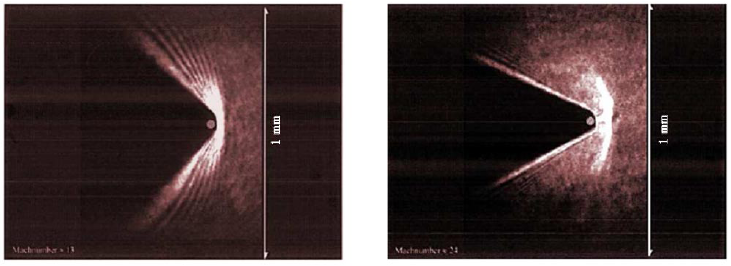
\includegraphics[width=.9\linewidth]{mach_number}
  \caption{
    % 
    Density profiles of an expanding BEC hitting a stationary defect
created by the repulsive potential of a blue-detuned laser beam. The
condensate has different speeds in the two panels, moving roughly
twice as fast in the right-panel. Notice the Mach cone formed behind
the defect, which gets narrower as the condesate moves faster. From
Ref.~\cite{Carusotto_2006}.
    % 
}\label{fig:mach-number}
\end{figure}
% 
\begin{figure}[tb]\centering
  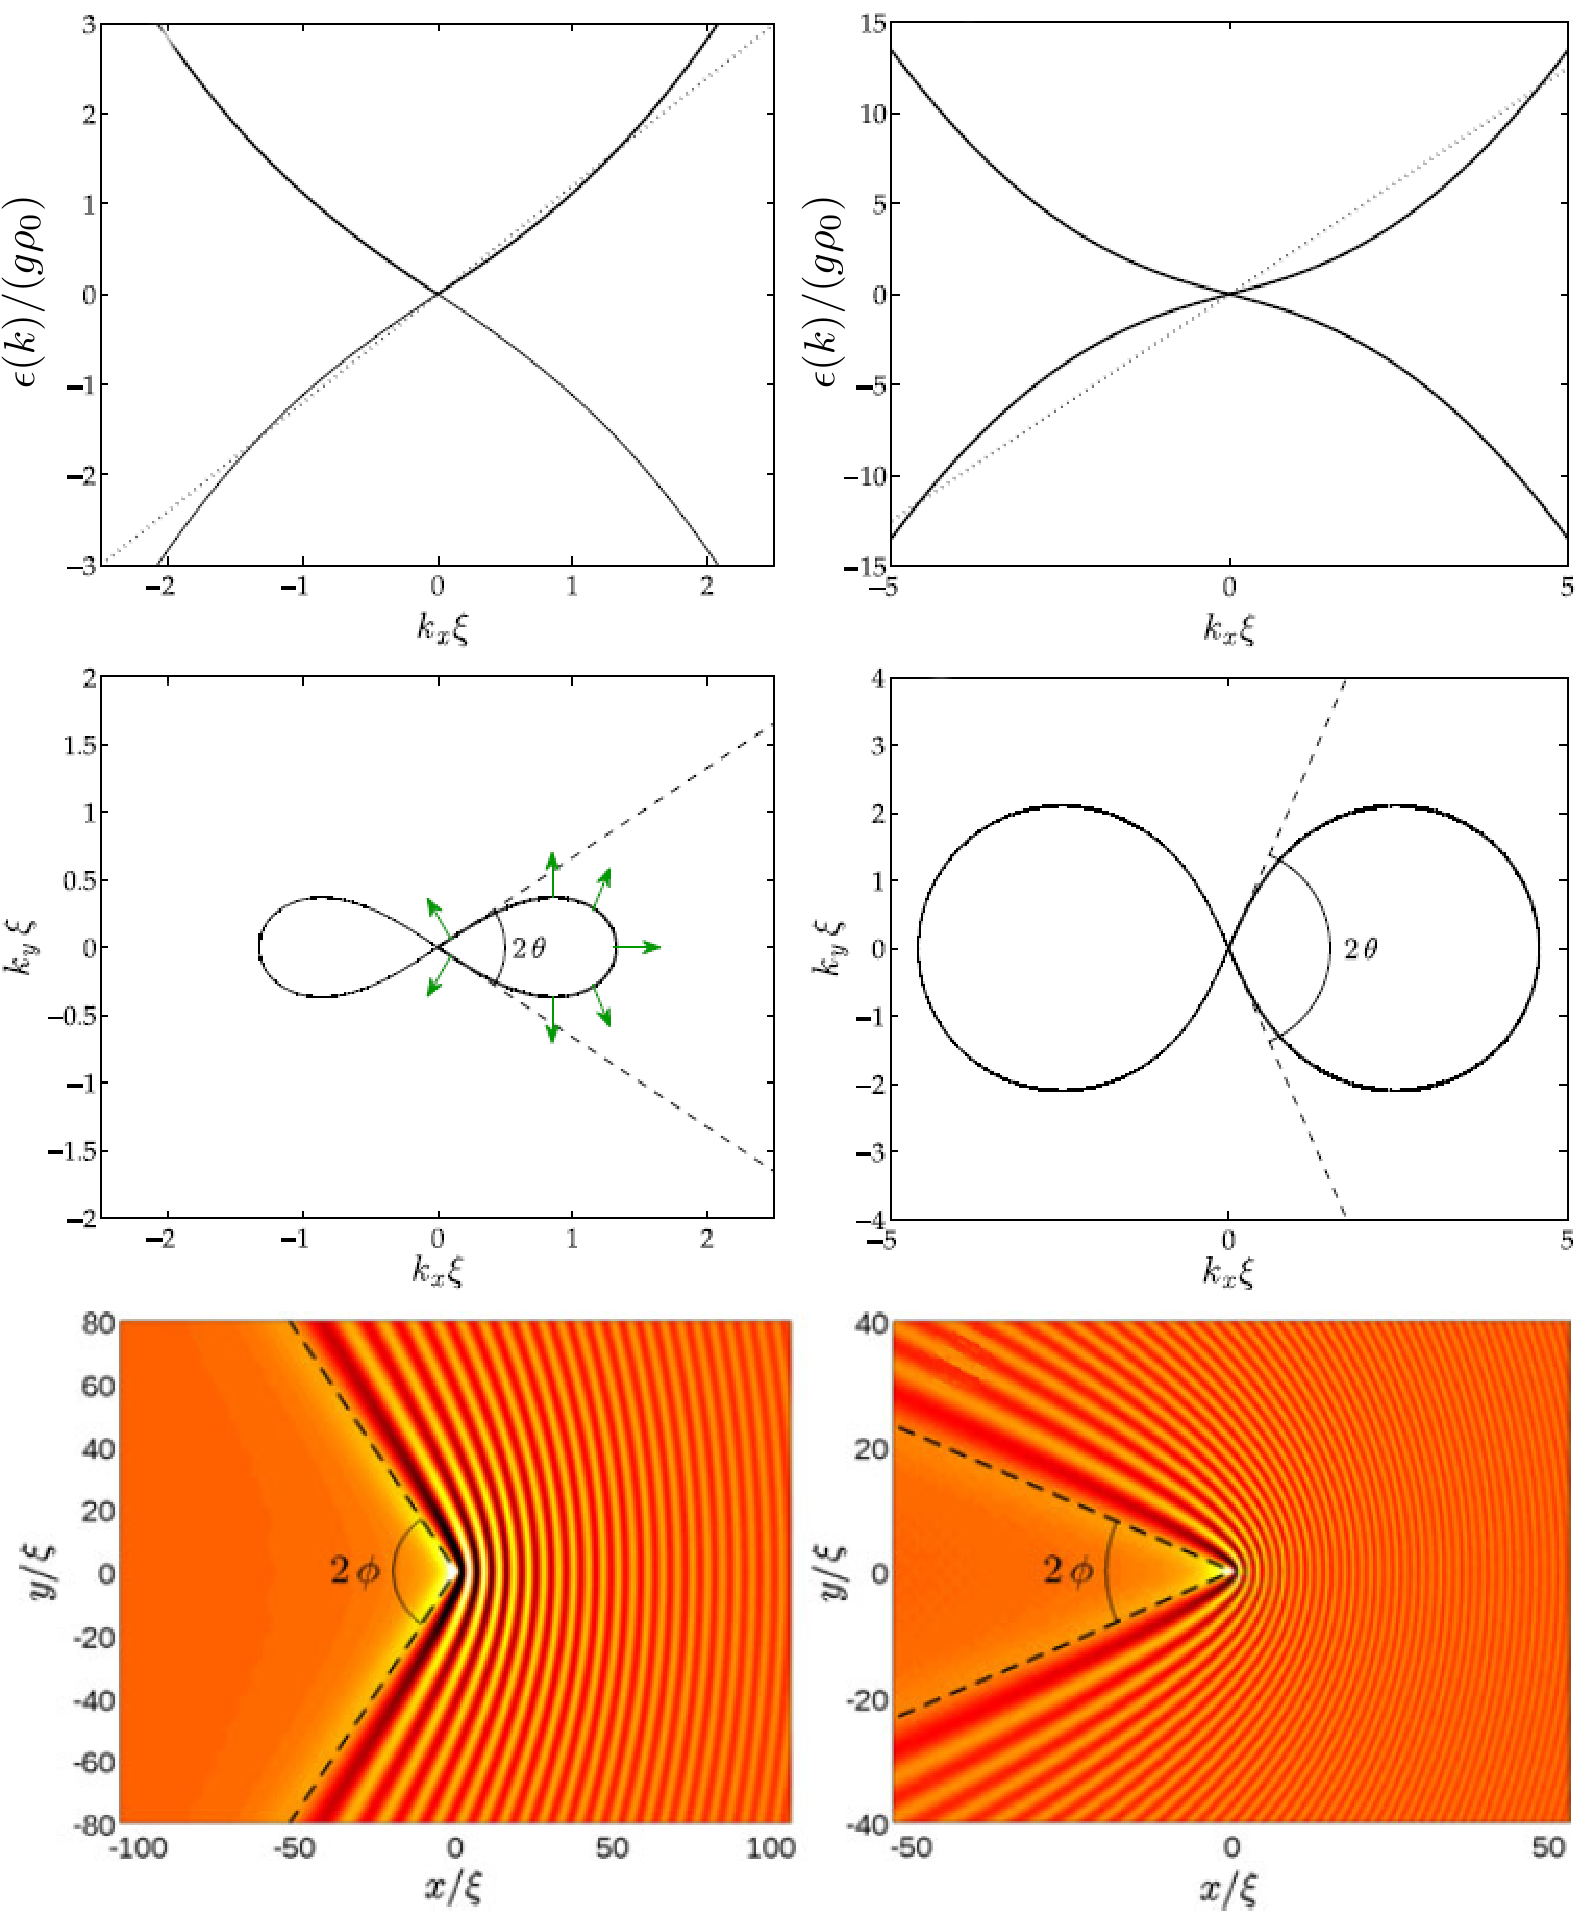
\includegraphics[width=.85\linewidth]{ducks_new}
  \caption{
    % 
    \emph{Top panels:} Bogoliubov dispersion
Eq.~\eqref{eq:bogoliubov}. The dotted lines indicate the $\bm{v}_0
\kv$ plane.
    \emph{Middle panels:} Locus $\Gamma$ of intersection of the 2D
dispersion with the $\bm{v}_0 \kv$ plane. Green arrows are normal
to $\Gamma$, while the dashed lines indicate the Cherenkov
cone.
    \emph{Bottom panels:} Real-space density modulation, with a
$\delta$--defect at $(0,0)$. Dashed lines show the Mach cone. Left
column panels are for $v_0 = 1.2 c_s$, and right column for $v_0 = 2.5
c_s$. From Ref.~\cite{9783319002651}.
    % 
}\label{fig:bogo-cherenkov}
\end{figure}

Using Eq.~\eqref{eq:atom-MF}, the GP Hamiltonian becomes
$H_{\text{GP}} = -\frac{\nabla^2}{2m} - \frac{k_0^2}{2m}$ and the
source term
$S(\rv) = \psi_0 V_d(\rv) \exp \left( i \bm{k_0} \rv \right)$. We now
get the linear operator for our problem in the form
%
\begin{equation}\label{eq:ourL}
  \Lca = \mat{-\frac{\nabla^2}{2m} - \frac{k_0^2}{2m} + g\rho_0}{g N_0 \psi_0^2 \exp \left( 2 i \bm{k_0} \rv \right)}{- g N_0 \psi_0^{\star 2} \exp \left( - 2 i \bm{k_0} \rv \right)}{-\left[ -\frac{\nabla^2}{2m} - \frac{k_0^2}{2m} + g\rho_0 \right]}
\end{equation}
% 
Notice that, due to the presence of the off-diagonal exponential
terms, $\Lca$ does not commute with the momentum operator, which is
the generator of the spatial translation group. Luckily, however, we
can restore translational invariance by a simple unitary
transformation, as shown below.

First, a brief reminder of basic quantum mechanics. Using the standard
commutation relations, one can show that, for a constant wavevector
$\bm{k_0}$, the unitary operator\footnote{The hat symbol denotes
  operators in the relevant Hilbert space.}
%
\begin{equation}\label{eq:trans-oper}
  \hat{T}(\bm{k_0}) = \exp \left( -i \bm{k_0} \hat{\rv} \right)
\end{equation}
% 
performs a translation in momentum space,
$\hat{T}(\bm{k_0}) \ket{\bm{k}} = \ket{\bm{k} - \bm{k_0}}$, with the
ket $\ket{\bm{k}}$ representing a single particle state with
wavevector $\bm{k}$ such that
$\hat{\bm{k}} \ket{\bm{k}} = \bm{k} \ket{\bm{k}}$. Using the
definitions above, one can easily obtain the commutator
%
\begin{equation}\label{eq:trans-commutator}
  \left[ \hat{\bm{k}},\, \hat{T}(\bm{k_0}) \right] = -\bm{k_0}\hat{T}(\bm{k_0}) 
\end{equation}
% 
This allows us to rewrite the following expressions
\begin{align}\label{eq:products}
  \begin{split}
    \hat{T}^{\dagger}(\bm{k_0})\hat{\bm{k}}\hat{T}(\bm{k_0})& = \hat{\bm{k}} - \bm{k_0}\hat{\mathbb{I}}\\
    \hat{T}(\bm{k_0})\hat{\bm{k}}\hat{T}^{\dagger}(\bm{k_0})& = \hat{\bm{k}} + \bm{k_0}\hat{\mathbb{I}}  
  \end{split}
\end{align}

We now recognize the two exponentials in Eq.~\eqref{eq:ourL} as being
the real-space representation of $\hat{T}^2(\bm{k_0})$ and its
hermitian conjugate. This motivates us to define the following unitary
operator
%
\begin{equation}\label{eq:ucal}
  \hat{\mathcal{T}}(\bm{k_0}) = \mat{\hat{T}(\bm{k_0})}{0}{0}{\hat{T}^{\dagger}(\bm{k_0})}
\end{equation}
% 
such that a unitary transformation of our operator $\Lca$ now restores translational
symmetry. Indeed, one can see that
%
\begin{equation}\label{eq:translated-L}
  \hat{\mathcal{T}} \hat{\Lca} \hat{\mathcal{T}}^{\dagger} = \mat{\frac{\left(\kop + \bm{k_0}\right)^2}{2m} - \frac{k_0^2}{2m} + g\rho_0}{g N_0 \psi_0^2}{- g N_0 \psi_0^{\star 2}}{-\left[\frac{\left(\kop - \bm{k_0}\right)^2}{2m} - \frac{k_0^2}{2m} + g\rho_0 \right]}
\end{equation}
% 
where we have made use of Eqs.~\eqref{eq:products} and we have written
$\hat{\Lca}$ in a base-independent representation.  In the subspace of
momentum eigenstates $\ket{\kv}$, we can write the (right-)eigenvalue
equation corresponding to Eq.~\eqref{eq:translated-L} as
%
\begin{equation}\label{eq:right-eigen}
  \Lca_{\text{GP}} [k] \colvec{U_\sigma(k)}{V_\sigma(k)} = \epsilon_\sigma(k) \colvec{U_\sigma(k)}{V_\sigma(k)}
\end{equation}
% 
where we have recovered the matrix representation of
Eq.~\eqref{eq:LGP}, and introduced the notation
$\omega_\sigma(\kv) = \bm{v}_0 \kv + \epsilon_\sigma(k)$. Here
$\sigma = \pm$ labels the 2 different eigenmodes, and we defined the
condensate speed $\bm{v}_0 \equiv \frac{\kv_0}{m}$.

Notice that the $k=0$ mode has only one eigenvector. However, one can
safely exclude it as this mode does not imply energy or momentum
transport. Excluding the $k = 0$ point, one can then solve
Eq.~\eqref{eq:right-eigen}, obtaining the celebrated Bogoliubov
excitation spectrum
%
\begin{equation}\label{eq:bogoliubov}
  \epsilon_\sigma(k) = \sigma \left[\frac{k^2}{2m}\left(\frac{k^2}{2m} + 2 g \rho_0 \right) \right]^{\frac{1}{2}}
\end{equation}
% 
with $\sigma = \pm$. Here $k$ represents the momentum of the
quasiparticle excitation with respect to the momentum $k_0$ of the
condensate. Note that the complex amplitudes $U_\sigma(k)$ and
$V_\sigma(k)$ only depend on the absolute value of $\kv$, while the
(real) spectrum of Eq.~\eqref{eq:translated-L}, $\omega_\sigma(\kv)$,
is the Bogoliubov spectrum with an additional Galilean boost
$\bm{v}_0 \kv$.

We can now further simplify the problem. As can be seen from
Eq.~\eqref{eq:symmetry-2}, the 2 eigen-families $\sigma$ and $-\sigma$
are linked by a duality, stemming from the $\mathcal{P} \mathcal{T}$
symmetry\footnote{This can be actually formally proven after defining
  the parity and time-reversal operators corresponding to our
  problem. For details, see Ref.~\cite{MOSTAFAZADEH_2010}.} of the
Bogoliubov operator $\Lca$.  We therefore drop the subscript $\sigma$
and make the convention that
$\left( U,\, V \right) \equiv \left( U_{+},\, V_{+} \right)$.

\paragraph{Bogoliubov spectrum discussion}
The Bogoliubov spectrum Eq.~\eqref{eq:bogoliubov} is shown in the top
row of Fig.~\ref{fig:bogo-cherenkov}, for two different values of
$v_0$, which sets the slope of the dotted lines (indicating the
$\bm{v}_0 \kv$ plane). In the non-interacting case $g=0$ and the
spectrum reduces to a simple parabola characterising a free
particle. For repulsive interactions, $g > 0$ and we can distinguish
two qualitatively different domains, after first introducing the
typical length scale of the problem, called the \textit{healing
  length}. The healing length $\xi$ is a measure of the distance over
which the condensate density recovers its equilibrium value $\rho_0$
when forced to vary away from this value. For example, in a box the
boundary conditions fix the density to zero at the positions of the
walls. In mathematical terms,
%
\begin{equation}\label{eq:healing-length}
  \frac{1}{m\xi^2}=g\rho_0
\end{equation}
% 

We first explore the domain of small momenta, $k\xi \ll 1$, which is
characterised by a linear behaviour of the dispersion,
$\epsilon(k) \simeq k c_s$, that implies the propagation of low-energy
excitations in the form of \textit{sound waves}, with a
velocity\footnote{The sound velocity here is measured in the
  condensate rest-frame ($k_0 = 0$).} $c_s$ given by
%
\begin{equation}\label{eq:sound-velocity}
  mc^2_s = g \rho_0
\end{equation}
% 
The \textit{Landau criterion} for superfluidity~\cite{9780198507192}
determines the maximum velocity at which a weak impurity can travel
through the condensate without dissipating energy. In order for it to
dissipate energy, such an impurity must be able to create
quasiparticle excitations in the condensate. Conservation of energy
then results in a critical velocity
%
\begin{equation}\label{eq:Landau}
  v_c=\min_{k} \left[\frac{\epsilon(k)}{k}\right]
\end{equation}
% 
below which no dissipation can occur. In our case, this velocity is
precisely equal to the speed of sound, $v_c =
c_s$. Furthermore, the two situations, the one of a particle moving
through the condensate, or of the condensate moving against a fixed
defect, are physically equivalent, being connected by a Galilean
transformation. We can therefore conclude that we must have
$v_0 \geq c_s$ in order to observe any propagating
perturbation. Before moving on, it is worth noting that the Landau
criterion has some asociated caveats. The first one is that we are
completely neglecting the nucleation of vortices by a macroscopic
defect with a size comparable to the healing length, which would lower
the effective critical velocity. Vortices would furthermore also break
the translational invariance along the transverse directions, an
invariance that we already made use of. The second caveat is that
quantum fluctuations are also neglected. As seen in
Ref.~\cite{Astrakharchik_2004}, they could lead to nonzero dissipation
even at sub-sonic speeds.

The second domain of interest is the one of large momenta,
$k\xi \gg 1$. Looking at Eq.~\eqref{eq:right-eigen}, one notices that
the only $k$-dependent parts of $\Lca_{\text{GP}} [k]$ are the
diagonal terms. These terms have opposite sign, so the off-diagonal
coupling between $U(k)$ and $V(k)$ becomes highly off-resonant at
large $k$. Completely neglecting it gives the free-particle-like
shifted parabola $\epsilon(k) \simeq k^2/(2m)+g\rho_0$, with
$U(k) \simeq 1$ and $V(k) \simeq 0$.
%
The discontinuity in the spectrum at zero momentum can be explained by
the fact that the diagonal and off-diagonal parts of $\Lca_{\text{GP}}
[0]$ are equal in absolute value.

In order to obtain the defect-induced density perturbation, we must
now also determine the eigenvectors of the problem. Making use of
Eq.~\eqref{eq:symmetry-1}, we can act with $\sigma_3$ on the
eigenstates of $\Lca_{\text{GP}}$ to obtain the ones of
$\Lca_{\text{GP}}^{\dagger}$. This finally leads us to a biorthonormal
basis
$\left\{ \ket{\psi_\sigma^R(\kv)},\, \ket{\psi_\sigma^L(\kv)}
\right\}$, containing 4 basis vectors
%
\begin{equation}\label{eq:biorthobasis}
  \left\{ \colvec{U(k)}{V(k)}, \colvec{V^{\star}(k)}{U^{\star}(k)}, \colvec{U(k)}{-V(k)}, \colvec{-V^{\star}(k)}{U^{\star}(k)} \right\} \bigotimes \ket{\kv}
\end{equation}
% 
which fulfill the orthonormality condition
%
\begin{equation}\label{eq:binormality}
  \braket{\psi_{\sigma^{\prime}}^L(\kv^{\prime})}{\psi_\sigma^R(\kv)} = \delta_{\sigma,\sigma^{\prime}} \delta^2(\kv - \kv^{\prime})
\end{equation}
% 
and the completeness relation
%
\begin{equation}\label{eq:bicompleteness}
  \sum_{\sigma = \pm} \int d^2 \kv \; \ket{\psi_\sigma^R(\kv)}\bra{\psi_\sigma^L(\kv)} = 1
\end{equation}
% 
provided of course that we normalize in such a way that
$\abs{U(k)}^2 - \abs{V(k)}^2 = 1$. In this basis, the spectral
decomposition of Eq.~\eqref{eq:translated-L} is the diagonal form
%
\begin{equation}\label{eq:bidecomposition}
  \hat{\mathcal{T}} \hat{\Lca} \hat{\mathcal{T}}^{\dagger} = \sum_{\sigma = \pm} \int d^2 \kv \; \omega_\sigma(\kv) \ket{\psi_\sigma^R(\kv)}\bra{\psi_\sigma^L(\kv)}
\end{equation}
% 
The concrete form of $\Lca_{\text{GP}}[k]$, coupled with the
normalization condition Eq.~\eqref{eq:norms}, determines the
eigenvectors of the ``+'' family up to a phase factor. Indeed, one can
choose $\abs{U(k)} \pm \abs{V(k)} = f(k)^{\pm\frac{1}{4}}$, with 
%
\begin{equation}
  f(k) = \frac{k^2/(2m)}{k^2/(2m) + 2g\rho_0}
\end{equation}
% 
Furthermore, in case the Hamiltonian doesn't contain any time-reversal
symmetry-breaking terms, one can chose $U(k)$ and $V(k)$ to be real
quantities, without loss of generality.

It is now a trivial matter to solve the linearized evolution equation
Eq.~\eqref{eq:GP-atoms-system}. In particular, for a localized static
defect potential $V_d(\rv) = g_V \delta^2(\rv)$, quasiparticle modes
at all wavevectors $k$ are excited.\footnote{If one wishes to
  selectively excite a pair of modes, one can use a periodic
  potential, following, for example, Ref.~\cite{Ianeselli_2006}.} The
source term is time-independent, and hence the quasi-particle
amplitudes of Eq.~\eqref{eq:amplitudes-bk} have the simple form
$b(\kv) = -s(\kv)/\omega(\kv)$. Equivalently, we can obtain the
defect-induced perturbation of the wavefunction from its initial
steady state by directly inverting Eq.~\eqref{eq:bidecomposition} and
then reversing the unitary transformation that was applied to obtain
Eq.~\eqref{eq:translated-L}. Whichever route we take, it is clear that
the final answer will have a resonant structure, containing
$\omega(\kv)$ in the denominator, hence the dominant modes will be the
ones that satisfy $\omega(\kv) = 0$.

\paragraph{Landau causality rule}
We must also touch on the subject of \textit{adiabatic switching} at
this point. Adiabatic switching is neccesary to causally distinguish
the past from the future, making sure that the time $t = -\infty$ is
prior to that of the occurence of any cause (in our case the defect)
giving rise to the effect (pertubation of the condensate density). The
way to achieve this in practice is by shifting the real poles of the
Bogoliubov dispersion Eq.~\eqref{eq:bogoliubov} into the lower half of
the complex plane by an infinitesimal amount,
$\epsilon(k) \rightarrow \epsilon(k) - i0^{+}$. This corresponds to a
weak damping of the plane wave solution and ensures that no Bogoliubov
excitations were present at $t = - \infty$.

We show the defect-induced perturbation of the condensate density in
the bottom row of Fig.~\ref{fig:bogo-cherenkov}, for two distinct
values of the condensate speed $v_0$. Rather than giving its full
analytical expression, it is more instructive to present a geometrical
construction, detailed in Ref.~\cite{9783319002651}, that can shed
light on the main features of the condensate response. 

\paragraph{Geometrical construction}
We have already identified the importance of the poles of
$\omega(\kv)$; the solutions of $\epsilon(k) + \bm{v}_0 \kv = 0$ can
be visualized if one plots the intersection of the Bogoliubov
dispersion surface $\epsilon(k)$ with the $\bm{v}_0 \kv$ plane. The
locus of this intersection is a closed curve that we will denote by
$\Gamma$ and that is plotted in the middle row of
Fig.~\ref{fig:bogo-cherenkov}. Making the connection with the Landau
criterion presented earlier, we can identify two regimes. 

For small velocities $v_0 < c_s$ we have the \textit{sub-sonic}
regime, where $\Gamma$ is a single point at the origin. Consequently,
one can observe superfluid-like behaviour with no propagating density
modulation. The modulation will stay localized in the vecinity of the
defect, and, in the Galilean-equivalent problem of a particle moving
through the condensate, it would renormalize the particle
mass.~\cite{Astrakharchik_2004}

As we gradually increases the condensate speed, and hence the slope of
the $\bm{v}_0 \kv$ plane, this plane will touch the surface of the
dispersion relation when $v_0 = c_s$, marking the entry into the
\textit{super-sonic} (dissipative) regime. Further increasing the
speed will increase the size of $\Gamma$, as can be seen in
Fig.~\ref{fig:bogo-cherenkov}. The green arrows, orthogonal to the
curve $\Gamma$ at each point, represent the group velocity of the
Bogoliubov mode at that particular $k$-value. They show the direction
of propagation of the density perturbation away from the defect, up to
infinity. It is the interference of these propagating modes that we
see as the real-space density pattern. Note that the locus $\Gamma$
has two distinct regions, inherited from the linear and quadratic
domains of the dispersion Eq.~\eqref{eq:bogoliubov}.

The linear region of $\Gamma$, close to the origin, is characterised
by essentially the same physics as the Cherenkov effect in
non-dispersive media. We remind the reader that the Charenkov effect
consists in the emission of electromagnetic radiation by a charged
particle moving relativistically through a dielectric medium at a
velocity higher than the (phase) velocity of light in that medium. The
emission is concentrated into a \textit{Cherenkov cone} in momentum
space, of aperture $2\theta$, where
$\cos\theta = c/v$.~\cite{jelley1958vcerenkov} The higher the particle
speed $v$ with respect to the speed of light $c$, the wider the angle
$\theta$ between the emission and the direction of motion. The
Cherenkov cone is depicted by the dashed lines in the middle panels of
Fig.~\ref{fig:bogo-cherenkov}, and the angle $\theta$ in our case is
of course given by $\cos\theta = c_s/v_0$. Due to the momentum-space
singularity at the origin, the group velocity has a jump, defining a
whole region of space where no phonons are emitted. This corresponds
in real-space to the so-called \textit{Mach cone}, named in analogy to
the cone that is created by a super-sonic aircraft (since we are
dealing with terminology, it is worth noting that the ratio $v_0/c_s$
goes by the name of \textit{Mach number}). The Mach cone is depicted
by dashed lines in the bottom panels of Fig.~\ref{fig:bogo-cherenkov}:
as its aperture $2\phi$ is quantified by $\sin\phi = c_s/v_0$, that
means that, the faster the fluid, the narrower the cone will be.

The high-momentum, rounded region of $\Gamma$, which corresponds to
the single-particle-like dispersion, has no equivalent in Cherenkov
physics. It is responsible for the hyperbolic-like
wavefronts\footnote{The wavefronts are actually parabolic in the
  non-interacting limit of $g=0$.}, emitted in the positive
$\hat{\bm{x}}$ direction. The physical origin of these rounded waves
lies in the interference between the coherent matter wave of the BEC
and the wave scattered off the defect. It it worth noting that the
curve $\Gamma$ also helps one determine the spacing between the
emitted wavefronts, which is inversely proportional to the value of
the momentum at the particular point on $\Gamma$ that corresponds to
the wave propagation direction. In practice, we see for example that
the spacing along $y = 0$, in the positive $\hat{\bm{x}}$ direction,
is wider in the left-bottom panel than in the right one.

Aside from being just a useful geometrical construction, the locus
$\Gamma$ can actually be observed in scattering experiments, both in
the context of atomic condensates, as well as for microcavity
polaritons (the topic of Chapter~\ref{cha:polaritons}), where it goes
by the name of Rayleigh scattering ring~\cite{Ciuti_2005}.



%TODO%
%%%%%%%%%%%%%%%%%%%%%%%%%%%%%%%%%%%%%%%%%%%%%%%%%%%%%%%%%%%%%%%%%%%%%%%%%%%%%%%%%%%%%%%%%%%%%%%%%%
% - global phase of the wavefunction in the time-independent(TI) GPE can                         %
%   be artitrarily chosen, U(1) symmetry                                                         %
% - U(1) symmetry of the MF eq                                                                   %
% - wavefunction of TIGPE is purely real in the absence of time-reversal symmetry breaking terms %
% - no macroscopic curent is flowing across the BEC in the GS                                    %
% - Goldstone mode (zero sound)                                                                  %
%%%%%%%%%%%%%%%%%%%%%%%%%%%%%%%%%%%%%%%%%%%%%%%%%%%%%%%%%%%%%%%%%%%%%%%%%%%%%%%%%%%%%%%%%%%%%%%%%%


%%% Local Variables:
%%% mode: latex
%%% TeX-master: "../thesis_berceanu"
%%% End:
